% *****************************************************************************************************
% ****************************             NUMERICAL ANALYSIS          ********************************
% *****************************************************************************************************

% =======================================================
% =======         HEADER FOR DOCUMENT        ============
% =======================================================

    % *********  SPECIFIC FOR THIS BOOK  ********
    \def\ProjectAuthorLink{https://github.com/CompilandoConocimiento}
    \def\ProjectNameLink{\ProjectAuthorLink/LibroAnalisisNumerico}    
    

    % *********   DOCUMENT ITSELF   **************
    \documentclass[12pt, fleqn]{report}                             %Type of doc and size of font and left equations
    \usepackage[margin=1.2in]{geometry}                             %Margins and Geometry pacakge
    \usepackage{ifthen}                                             %Allow simple programming using if - then
    \usepackage[hidelinks]{hyperref}                                %Allow to create hiperlinks and Fuck Firefox
    \usepackage{pdfpages}                                           %Allow us 'import' PDF's
    \hypersetup{pageanchor=false}                                   %Solve 'double page 1' warnings in build :v
    \setlength{\parindent}{0pt}                                     %Eliminate ugly indentation
    \author{Oscar Andrés Rosas}                                     %Who I am

    % *********   LANGUAJE    *****************
    \usepackage[spanish]{babel}                                     %Please allow me to type in spanish
    \usepackage[utf8]{inputenc}                                     %Lets use UFT-8
    \usepackage[T1]{fontenc}                                        %Allow for better font support
    \usepackage{textcmds}                                           %Allow us to use quoutes
    \usepackage{changepage}                                         %Allow us to use identate paragraphs
    \usepackage{anyfontsize}                                        %All the sizes for fonts wiiiii!

    % *********   MATH AND HIS STYLE  *********
    \usepackage{ntheorem, amsmath, amssymb, amsfonts}               %All fucking math, I want all!
    \usepackage{mathrsfs, mathtools, empheq}                        %All fucking math, I want all!
    \usepackage{cancel}                                             %Negate symbol
    \usepackage{centernot}                                          %Allow me to negate a symbol
    \decimalpoint                                                   %Use decimal point

    % *********   GRAPHICS AND IMAGES *********
    \usepackage{graphicx}                                           %Allow to create graphics
    \usepackage{float}                                              %For images
    \usepackage{wrapfig}                                            %Allow to create images
    \graphicspath{ {Graphics/} }                                    %Where are the images :D

    % *********   LISTS AND TABLES ***********
    \usepackage{listings, listingsutf8}                             %We will be using code here
    \usepackage[inline]{enumitem}                                   %We will need to enumarate
    \usepackage{tasks}                                              %Horizontal lists
    \usepackage{longtable}                                          %Lets make tables awesome
    \usepackage{booktabs}                                           %Lets make tables awesome
    \usepackage{tabularx}                                           %Lets make tables awesome
    \usepackage{multirow}                                           %Lets make tables awesome
    \usepackage{multicol}                                           %Create multicolumns

    % *********   REMOVE SOME ERRORS **********
    \hbadness=10000                                                 %Ignore \vbox and \hbox warings
    \hfuzz=\maxdimen\newdimen\hfuzz                                 %Ignore \vbox and \hbox warings

    % *********   HEADERS AND FOOTERS ********
    \usepackage{fancyhdr}                                           %Lets make awesome headers/footers
    \pagestyle{fancy}                                               %Lets make awesome headers/footers
    \setlength{\headheight}{16pt}                                   %Top line
    \setlength{\parskip}{0.5em}                                     %Top line
    \renewcommand{\footrulewidth}{0.5pt}                            %Bottom line

    \lhead {                                                        %Left Header
        \hyperlink{chapter.\arabic{chapter}}                        %Make a link to the current chapter
        {\normalsize{\textsc{\nouppercase{\leftmark}}}}             %And fot it put the name
    }

    \rhead {                                                        %Right Header
        \hyperlink{section.\arabic{chapter}.\arabic{section}}       %Make a link to the current chapter
            {\footnotesize{\textsc{\nouppercase{\rightmark}}}}      %And fot it put the name
    }

    \rfoot{\textsc{\small{\hyperref[sec:Index]{Ve al Índice}}}}     %This will always be a footer  

    \fancyfoot[L]{                                                  %Algoritm for a changing footer
        \ifthenelse{\isodd{\value{page}}}                           %IF ODD PAGE:
            {\href{https://SoyOscarRH.github.io/}                   %DO THIS:
                {\footnotesize                                      %Send the page
                    {\textsc{Oscar Andrés Rosas}}}}                 %Send the page
            {\href{https://compilandoconocimiento.com}              %ELSE DO THIS: 
                {\footnotesize                                      %Send the author
                    {\textsc{Compilando Conocimiento}}}}            %Send the author
    }
    
    
% =======================================================
% ===================   COMMANDS    =====================
% =======================================================

    % =========================================
    % =======   NEW ENVIRONMENTS   ============
    % =========================================
    \newenvironment{Indentation}[1][0.75em]                         %Use: \begin{Inde...}[Num]...\end{Inde...}
        {\begin{adjustwidth}{#1}{}}                                 %If you dont put nothing i will use 0.75 em
        {\end{adjustwidth}}                                         %This indentate a paragraph
    
    \newenvironment{SmallIndentation}[1][0.75em]                    %Use: The same that we upper one, just 
        {\begin{adjustwidth}{#1}{}\begin{footnotesize}}             %footnotesize size of letter by default
        {\end{footnotesize}\end{adjustwidth}}                       %that's it
    
    \def \Eq {equation}                                             %Stupid Visual studio error
    \newenvironment{MultiLineEquation}[1]                           %Use: To create MultiLine equations
        {\begin{\Eq}\begin{alignedat}{#1}}                          %Use: \begin{Multi..}{Num. de Columnas}
        {\end{alignedat}\end{\Eq}}                                  %And.. that's it!
    
    \newenvironment{MultiLineEquation*}[1]                          %Use: To create MultiLine equations
        {\begin{\Eq*}\begin{alignedat}{#1}}                         %Use: \begin{Multi..}{Num. de Columnas}
        {\end{alignedat}\end{\Eq*}}                                 %And.. that's it!

    \newenvironment{largeEq} {\begingroup \large}{\endgroup}        %Make eq bigger
    \newenvironment{LargeEq} {\begingroup \Large}{\endgroup}        %Make eq bigger
    \newenvironment{HugeEq} {\begingroup \Huge}{\endgroup}          %Make eq bigger!

    % =========================================
    % == GENERAL TEXT & SYMBOLS ENVIRONMENTS ==
    % =========================================
    
    % =====  TEXT  ======================
    \newcommand \Quote              {\qq}                           %Use: \Quote to use quotes
    \newcommand \Over               {\overline}                     %Use: \Bar to use just for short
    \newcommand \ForceNewLine       {$\Space$\\}                    %Use it in theorems for example
    \newcommand \ForceColumnBreak   {\vfill\null\columnbreak}       %Use only in multicols

    % =====  SPACES  ====================
    \DeclareMathOperator \Space     {\quad}                         %Use: \Space for a cool mega space
    \DeclareMathOperator \MegaSpace {\quad \quad}                   %Use: \MegaSpace for a cool mega mega space
    \DeclareMathOperator \MiniSpace {\;}                            %Use: \Space for a cool mini space
    
    % =====  MATH TEXT  =================
    \newcommand \Such           {\MiniSpace | \MiniSpace}           %Use: \Such like in sets
    \newcommand \Also           {\MiniSpace \text{y} \MiniSpace}    %Use: \Also so it's look cool
    \newcommand \Remember[1]    {\Space\text{\scriptsize{#1}}}      %Use: \Remember so it's look cool
    
    % =====  THEOREMS: IN SPANISH :0  ===
    \newtheorem{Theorem}        {Teorema}[section]                  %Use: \begin{Theorem}[Name]\label{Nombre}...
    \newtheorem{Corollary}      {Colorario}[Theorem]                %Use: \begin{Corollary}[Name]\label{Nombre}...
    \newtheorem{Lemma}[Theorem] {Lemma}                             %Use: \begin{Lemma}[Name]\label{Nombre}...
    \newtheorem{Definition}     {Definición}[section]               %Use: \begin{Definition}[Name]\label{Nombre}...
    \theoremstyle{break}                                            %THEOREMS START 1 SPACE AFTER Fuck!

    % =====  LOGIC  =====================
    \newcommand \lIff    {\leftrightarrow}                          %Use: \lIff for logic iff
    \newcommand \lEqual  {\MiniSpace \Leftrightarrow \MiniSpace}    %Use: \lEqual for a logic double arrow
    \newcommand \lInfire {\MiniSpace \Rightarrow \MiniSpace}        %Use: \lInfire for a logic infire
    \newcommand \lLongTo {\longrightarrow}                          %Use: \lLongTo for a long arrow
    \newcommand \lAnd    {\land}                                    %Use: \lAnd ^
    \newcommand \lOr     {\lor}                                     %Use: \lOr or symbol
    \newcommand \lNot    {\neg}                                     %Use: \lNot for negation

    % =====  FAMOUS SETS  ===============
    \DeclareMathOperator \Naturals     {\mathbb{N}}                 %Use: \Naturals por Notation
    \DeclareMathOperator \Primes       {\mathbb{P}}                 %Use: \Primes por Notation
    \DeclareMathOperator \Integers     {\mathbb{Z}}                 %Use: \Integers por Notation
    \DeclareMathOperator \Racionals    {\mathbb{Q}}                 %Use: \Racionals por Notation
    \DeclareMathOperator \Reals        {\mathbb{R}}                 %Use: \Reals por Notation
    \DeclareMathOperator \Complexs     {\mathbb{C}}                 %Use: \Complex por Notation
    \DeclareMathOperator \GenericField {\mathbb{F}}                 %Use: \GenericField por Notation
    \DeclareMathOperator \VectorSet    {\mathbb{V}}                 %Use: \VectorSet por Notation
    \DeclareMathOperator \SubVectorSet {\mathbb{W}}                 %Use: \SubVectorSet por Notation
    \DeclareMathOperator \Polynomials  {\mathbb{P}}                 %Use: \Polynomials por Notation
    \DeclareMathOperator \VectorSpace  {\VectorSet_{\GenericField}} %Use: \VectorSpace por Notation
    \DeclareMathOperator \LinealTransformation {\mathcal{T}}        %Use: \LinealTransformation for a cool T
    \DeclareMathOperator \LinTrans      {\mathcal{T}}               %Use: \LinTrans for a cool T
    \DeclareMathOperator \Laplace       {\mathcal{L}}               %Use: \LinTrans for a cool T

    % =====  CONTAINERS   ===============
    \newcommand{\Set}[1]            {\left\{ \; #1 \; \right\}}     %Use: \Set {Info} for INTELLIGENT space 
    \newcommand{\bigSet}[1]         {\big\{  \; #1 \; \big\}}       %Use: \bigSet  {Info} for space 
    \newcommand{\BigSet}[1]         {\Big\{  \; #1 \; \Big\}}       %Use: \BigSet  {Info} for space 
    \newcommand{\biggSet}[1]        {\bigg\{ \; #1 \; \bigg\}}      %Use: \biggSet {Info} for space 
    \newcommand{\BiggSet}[1]        {\Bigg\{ \; #1 \; \Bigg\}}      %Use: \BiggSet {Info} for space 
        
    \newcommand{\Wrap}[1]           {\left( #1 \right)}             %Use: \Wrap {Info} for INTELLIGENT space
    \newcommand{\bigWrap}[1]        {\big( \; #1 \; \big)}          %Use: \bigBrackets  {Info} for space 
    \newcommand{\BigWrap}[1]        {\Big( \; #1 \; \Big)}          %Use: \BigBrackets  {Info} for space 
    \newcommand{\biggWrap}[1]       {\bigg( \; #1 \; \bigg)}        %Use: \biggBrackets {Info} for space 
    \newcommand{\BiggWrap}[1]       {\Bigg( \; #1 \; \Bigg)}        %Use: \BiggBrackets {Info} for space 

    \newcommand{\Brackets}[1]       {\left[ #1 \right]}             %Use: \Brackets {Info} for INTELLIGENT space
    \newcommand{\bigBrackets}[1]    {\big[ \; #1 \; \big]}          %Use: \bigBrackets  {Info} for space 
    \newcommand{\BigBrackets}[1]    {\Big[ \; #1 \; \Big]}          %Use: \BigBrackets  {Info} for space 
    \newcommand{\biggBrackets}[1]   {\bigg[ \; #1 \; \bigg]}        %Use: \biggBrackets {Info} for space 
    \newcommand{\BiggBrackets}[1]   {\Bigg[ \; #1 \; \Bigg]}        %Use: \BiggBrackets {Info} for space 

    \newcommand{\Generate}[1]   {\left\langle #1 \right\rangle}     %Use: \Generate {Info} <>
    \newcommand{\Floor}[1]      {\left \lfloor #1 \right \rfloor}   %Use: \Floor {Info} for floor 
    \newcommand{\Ceil}[1]       {\left \lceil #1 \right \rceil }    %Use: \Ceil {Info} for ceil
    
    % =====  BETTERS MATH COMMANDS   =====
    \newcommand{\pfrac}[2]      {\Wrap{\dfrac{#1}{#2}}}             %Use: Put fractions in parentesis
    \newcommand{\Sum}           {\displaystyle \sum}                %Use: Sum to big sum
    \newcommand{\Int}           {\displaystyle \int}                %Use: Sum to big integral


    % =========================================
    % ====   LINEAL ALGEBRA & VECTORS    ======
    % =========================================

    % ===== UNIT VECTORS  ================
    \newcommand{\hati}      {\hat{\imath}}                           %Use: \hati for unit vector    
    \newcommand{\hatj}      {\hat{\jmath}}                           %Use: \hatj for unit vector    
    \newcommand{\hatk}      {\hat{k}}                                %Use: \hatk for unit vector

    % ===== MAGNITUDE  ===================
    \newcommand{\abs}[1]    {\left\lvert #1 \right\lvert}           %Use: \abs{expression} for |x|
    \newcommand{\Abs}[1]    {\left\lVert #1 \right\lVert}           %Use: \Abs{expression} for ||x||
    \newcommand{\Mag}[1]    {\left| #1 \right|}                     %Use: \Mag {Info} 
    
    \newcommand{\bVec}[1]   {\mathbf{#1}}                           %Use for bold type of vector
    \newcommand{\lVec}[1]   {\overrightarrow{#1}}                   %Use for a long arrow over a vector
    \newcommand{\uVec}[1]   {\mathbf{\hat{#1}}}                     %Use: Unitary Vector Example: $\uVec{i}

    % ===== FN LINEAL TRANSFORMATION  ====
    \newcommand{\FnLinTrans}[1]{\mathcal{T}\Wrap{#1}}               %Use: \FnLinTrans for a cool T
    \newcommand{\VecLinTrans}[1]{\mathcal{T}\pVector{#1}}           %Use: \LinTrans for a cool T
    \newcommand{\FnLinealTransformation}[1]{\mathcal{T}\Wrap{#1}}   %Use: \FnLinealTransformation

    % ===== ALL FOR DOT PRODUCT  =========
    \makeatletter                                                   %WTF! IS THIS
    \newcommand*\dotP{\mathpalette\dotP@{.5}}                       %Use: \dotP for dot product
    \newcommand*\dotP@[2] {\mathbin {                               %WTF! IS THIS            
        \vcenter{\hbox{\scalebox{#2}{$\m@th#1\bullet$}}}}           %WTF! IS THIS
    }                                                               %WTF! IS THIS
    \makeatother                                                    %WTF! IS THIS

    % === WRAPPERS FOR COLUMN VECTOR ===
    \newcommand{\pVector}[1]                                        %Use: \pVector {Matrix Notation} use parentesis
        { \ensuremath{\begin{pmatrix}#1\end{pmatrix}} }             %Example: \pVector{a\\b\\c} or \pVector{a&b&c} 
    \newcommand{\lVector}[1]                                        %Use: \lVector {Matrix Notation} use a abs 
        { \ensuremath{\begin{vmatrix}#1\end{vmatrix}} }             %Example: \lVector{a\\b\\c} or \lVector{a&b&c} 
    \newcommand{\bVector}[1]                                        %Use: \bVector {Matrix Notation} use a brackets 
        { \ensuremath{\begin{bmatrix}#1\end{bmatrix}} }             %Example: \bVector{a\\b\\c} or \bVector{a&b&c} 
    \newcommand{\Vector}[1]                                         %Use: \Vector {Matrix Notation} no parentesis
        { \ensuremath{\begin{matrix}#1\end{matrix}} }               %Example: \Vector{a\\b\\c} or \Vector{a&b&c}

    % === MAKE MATRIX BETTER  =========
    \makeatletter                                                   %Example: \begin{matrix}[cc|c]
    \renewcommand*\env@matrix[1][*\c@MaxMatrixCols c] {             %WTF! IS THIS
        \hskip -\arraycolsep                                        %WTF! IS THIS
        \let\@ifnextchar\new@ifnextchar                             %WTF! IS THIS
        \array{#1}                                                  %WTF! IS THIS
    }                                                               %WTF! IS THIS
    \makeatother                                                    %WTF! IS THIS
    
    \newcommand{\adotP}[2] {\left< #1, #2 \right> }                 %Use for <x, y>
    \newcommand{\wdotP}[2] {\Wrap{ #1, #2 } }                       %Use for (x, y)
    \newcommand{\cdotP}[2] {\Wrap{ #1 \dotP #2 } }                  %Use for (x * y)


    % =========================================
    % =======   FAMOUS FUNCTIONS   ============
    % =========================================

    % == TRIGONOMETRIC FUNCTIONS  ====
    \newcommand{\Cos}[1] {\cos\Wrap{#1}}                            %Simple wrappers
    \newcommand{\Sin}[1] {\sin\Wrap{#1}}                            %Simple wrappers
    \newcommand{\Tan}[1] {tan\Wrap{#1}}                             %Simple wrappers
    
    \newcommand{\Sec}[1] {sec\Wrap{#1}}                             %Simple wrappers
    \newcommand{\Csc}[1] {csc\Wrap{#1}}                             %Simple wrappers
    \newcommand{\Cot}[1] {cot\Wrap{#1}}                             %Simple wrappers

    % === COMPLEX ANALYSIS TRIG ======
    \newcommand \Cis[1]  {\Cos{#1} + i \Sin{#1}}                    %Use: \Cis for cos(x) + i sin(x)
    \newcommand \pCis[1] {\Wrap{\Cis{#1}}}                          %Use: \pCis for the same with parantesis
    \newcommand \bCis[1] {\Brackets{\Cis{#1}}}                      %Use: \bCis for the same with Brackets


    % =========================================
    % ===========     CALCULUS     ============
    % =========================================

    % ====== TRANSFORMS =============
    \newcommand{\FourierT}[1]   {\mathscr{F} \left\{ #1 \right\} }  %Use: \FourierT {Funtion}
    \newcommand{\InvFourierT}[1]{\mathscr{F}^{-1}\left\{#1\right\}} %Use: \InvFourierT {Funtion}

    % ====== DERIVATIVES ============
    \newcommand \MiniDerivate[1][x]   {\dfrac{d}{d #1}}             %Use: \MiniDerivate[var] for simple use [var]
    \newcommand \Derivate[2]          {\dfrac{d \; #1}{d #2}}       %Use: \Derivate [\Fun{x}][x]
    \newcommand \MiniUpperDerivate[2] {\dfrac{d^{#2}}{d#1^{#2}}}    %Mini Derivate High Orden Derivate -- [x][pow]
    \newcommand \UpperDerivate[3] {\dfrac{d^{#3} \; #1}{d#2^{#3}}}  %Complete High Orden Derivate -- [\Fun{x}][x][pow]
    
    \newcommand \MiniPartial[1][x] {\dfrac{\partial}{\partial #1}}  %Use: \MiniDerivate for simple use [var]
    \newcommand \Partial[2] {\dfrac{\partial \; #1}{\partial #2}}   %Complete Partial Derivate -- [\Fun{x}][x]
    \newcommand \MiniUpperPartial[2]                                %Mini Derivate High Orden Derivate -- [x][pow] 
        {\dfrac{\partial^{#2}}{\partial #1^{#2}}}                   %Mini Derivate High Orden Derivate
    \newcommand \UpperPartial[3]                                    %Complete High Orden Derivate -- [\Fun{x}][x][pow]
        {\dfrac{\partial^{#3} \; #1}{\partial#2^{#3}}}              %Use: \UpperDerivate for simple use

    \DeclareMathOperator \Evaluate  {\Big|}                         %Use: \Evaluate por Notation

    % ====== INTEGRALS ============
    \newcommand{\inftyInt} {\int_{-\infty}^{\infty}}                %Use: \inftyInt for simple integrants
    
        
% =======================================================
% ===========      COLOR: MATERIAL DESIGN     ===========
% =======================================================

    % =====  COLORS ==================
    \definecolor{RedMD}{HTML}{F44336}                               %Use: Color :D        
    \definecolor{Red100MD}{HTML}{FFCDD2}                            %Use: Color :D        
    \definecolor{Red200MD}{HTML}{EF9A9A}                            %Use: Color :D        
    \definecolor{Red300MD}{HTML}{E57373}                            %Use: Color :D        
    \definecolor{Red700MD}{HTML}{D32F2F}                            %Use: Color :D 

    \definecolor{PurpleMD}{HTML}{9C27B0}                            %Use: Color :D        
    \definecolor{Purple100MD}{HTML}{E1BEE7}                         %Use: Color :D        
    \definecolor{Purple200MD}{HTML}{EF9A9A}                         %Use: Color :D        
    \definecolor{Purple300MD}{HTML}{BA68C8}                         %Use: Color :D        
    \definecolor{Purple700MD}{HTML}{7B1FA2}                         %Use: Color :D 

    \definecolor{IndigoMD}{HTML}{3F51B5}                            %Use: Color :D        
    \definecolor{Indigo100MD}{HTML}{C5CAE9}                         %Use: Color :D        
    \definecolor{Indigo200MD}{HTML}{9FA8DA}                         %Use: Color :D        
    \definecolor{Indigo300MD}{HTML}{7986CB}                         %Use: Color :D        
    \definecolor{Indigo700MD}{HTML}{303F9F}                         %Use: Color :D 

    \definecolor{BlueMD}{HTML}{2196F3}                              %Use: Color :D        
    \definecolor{Blue100MD}{HTML}{BBDEFB}                           %Use: Color :D        
    \definecolor{Blue200MD}{HTML}{90CAF9}                           %Use: Color :D        
    \definecolor{Blue300MD}{HTML}{64B5F6}                           %Use: Color :D        
    \definecolor{Blue700MD}{HTML}{1976D2}                           %Use: Color :D        
    \definecolor{Blue900MD}{HTML}{0D47A1}                           %Use: Color :D  

    \definecolor{CyanMD}{HTML}{00BCD4}                              %Use: Color :D        
    \definecolor{Cyan100MD}{HTML}{B2EBF2}                           %Use: Color :D        
    \definecolor{Cyan200MD}{HTML}{80DEEA}                           %Use: Color :D        
    \definecolor{Cyan300MD}{HTML}{4DD0E1}                           %Use: Color :D        
    \definecolor{Cyan700MD}{HTML}{0097A7}                           %Use: Color :D        
    \definecolor{Cyan900MD}{HTML}{006064}                           %Use: Color :D 

    \definecolor{TealMD}{HTML}{009688}                              %Use: Color :D        
    \definecolor{Teal100MD}{HTML}{B2DFDB}                           %Use: Color :D        
    \definecolor{Teal200MD}{HTML}{80CBC4}                           %Use: Color :D        
    \definecolor{Teal300MD}{HTML}{4DB6AC}                           %Use: Color :D        
    \definecolor{Teal700MD}{HTML}{00796B}                           %Use: Color :D        
    \definecolor{Teal900MD}{HTML}{004D40}                           %Use: Color :D 

    \definecolor{GreenMD}{HTML}{4CAF50}                             %Use: Color :D        
    \definecolor{Green100MD}{HTML}{C8E6C9}                          %Use: Color :D        
    \definecolor{Green200MD}{HTML}{A5D6A7}                          %Use: Color :D        
    \definecolor{Green300MD}{HTML}{81C784}                          %Use: Color :D        
    \definecolor{Green700MD}{HTML}{388E3C}                          %Use: Color :D        
    \definecolor{Green900MD}{HTML}{1B5E20}                          %Use: Color :D

    \definecolor{AmberMD}{HTML}{FFC107}                             %Use: Color :D        
    \definecolor{Amber100MD}{HTML}{FFECB3}                          %Use: Color :D        
    \definecolor{Amber200MD}{HTML}{FFE082}                          %Use: Color :D        
    \definecolor{Amber300MD}{HTML}{FFD54F}                          %Use: Color :D        
    \definecolor{Amber700MD}{HTML}{FFA000}                          %Use: Color :D        
    \definecolor{Amber900MD}{HTML}{FF6F00}                          %Use: Color :D

    \definecolor{OrangeMD}{HTML}{ff9800}                            %Use: Color :D        
    \definecolor{Orange100MD}{HTML}{ffe0b2}                         %Use: Color :D        
    \definecolor{Orange200MD}{HTML}{ffcc80}                         %Use: Color :D        
    \definecolor{Orange300MD}{HTML}{ffb74d}                         %Use: Color :D        
    \definecolor{Orange700MD}{HTML}{fb8c00}                         %Use: Color :D        
    \definecolor{Orange900MD}{HTML}{ef6c00}                         %Use: Color :D

    \definecolor{BlueGreyMD}{HTML}{607D8B}                          %Use: Color :D        
    \definecolor{BlueGrey100MD}{HTML}{CFD8DC}                       %Use: Color :D        
    \definecolor{BlueGrey200MD}{HTML}{B0BEC5}                       %Use: Color :D        
    \definecolor{BlueGrey300MD}{HTML}{90A4AE}                       %Use: Color :D        
    \definecolor{BlueGrey700MD}{HTML}{455A64}                       %Use: Color :D        
    \definecolor{BlueGrey900MD}{HTML}{263238}                       %Use: Color :D        

    \definecolor{DeepPurpleMD}{HTML}{673AB7}                        %Use: Color :D

    % =====  ENVIRONMENT ==============
    \newcommand{\Color}[2]{\textcolor{#1}{#2}}                      %Simple color environment
    \newenvironment{ColorText}[1]                                   %Use: \begin{ColorText}
        { \leavevmode\color{#1}\ignorespaces }                      %That's is!


% =======================================================
% ===========           CODE EDITING          ===========
% =======================================================

    % =====  CODE EDITOR =============
    \lstdefinestyle{CompilandoStyle} {                              %This is Code Style
        backgroundcolor     = \color{BlueGrey900MD},                %Background Color  
        basicstyle          = \tiny\color{white},                   %Style of text
        commentstyle        = \color{BlueGrey200MD},                %Comment style
        stringstyle         = \color{Green300MD},                   %String style
        keywordstyle        = \color{Blue300MD},                    %keywords style
        numberstyle         = \tiny\color{TealMD},                  %Size of a number
        frame               = shadowbox,                            %Adds a frame around the code
        breakatwhitespace   = true,                                 %Style   
        breaklines          = true,                                 %Style   
        showstringspaces    = false,                                %Hate those spaces                  
        breaklines          = true,                                 %Style                   
        keepspaces          = true,                                 %Style                   
        numbers             = left,                                 %Style                   
        numbersep           = 10pt,                                 %Style 
        xleftmargin         = \parindent,                           %Style 
        tabsize             = 4,                                    %Style
        inputencoding       = utf8/latin1                           %Allow me to use special chars
    }

    % =====  CODE EDITOR =============
    \lstdefinestyle{CompilandoStylePurity} {                        %This is Code Style
        backgroundcolor     = \color{white},                        %Background Color  
        basicstyle          = \tiny\color{BlueGrey900MD},           %Style of text
        commentstyle        = \color{Green300MD},                   %Comment style
        stringstyle         = \color{Teal700MD},                    %String style
        keywordstyle        = \color{Blue700MD},                    %keywords style
        numberstyle         = \tiny\color{TealMD},                  %Size of a number
        frame               = none,                                 %Adds a frame around the code
        breakatwhitespace   = true,                                 %Style   
        breaklines          = true,                                 %Style   
        showstringspaces    = false,                                %Hate those spaces                  
        breaklines          = true,                                 %Style                   
        keepspaces          = true,                                 %Style                   
        numbers             = left,                                 %Style                   
        numbersep           = 11pt,                                 %Style 
        xleftmargin         = \parindent,                           %Style 
        tabsize             = 4,                                    %Style
        inputencoding       = utf8/latin1                           %Allow me to use special chars
    }
 
    \lstset{style = CompilandoStyle}                                %Use this style


% =======================================================
% ===========           VARIABLES             ===========
% =======================================================

    % =====  SOLVE LINEAL SYSTEM   =============

    \newcommand \ColorFun          {Red700MD}                       %Color definition
    \newcommand \ColorBigFun       {Teal700MD}                      %Color definition
    \newcommand \ColorFunG         {Orange900MD}                    %Color definition
    \newcommand \ColorFunDer       {Blue700MD}                      %Color definition
    \newcommand \ColorBigFunDer    {Blue700MD}                      %Color definition
    \newcommand \ColorFunDerDer    {Purple700MD}                    %Color definition
    \newcommand \ColorRoot         {Green700MD}                     %Color definition
    \newcommand \ColorVarA         {Purple700MD}                    %Color definition
    \newcommand \ColorVarB         {BlueGrey700MD}                  %Color definition
    \newcommand \ColorVarC         {Orange900MD}                    %Color definition
    \newcommand \ColorVarX         {Purple300MD}                    %Color definition
    \newcommand \ColorVarXpu       {Purple700MD}                    %Color definition
    \newcommand \ColorVarXmu       {Blue300MD}                      %Color definition
    \newcommand \ColorVarXOne      {Purple700MD}                    %Color definition
    \newcommand \ColorVarXTwo      {Blue700MD}                      %Color definition

    \newcommand \Fun[1]      {\Color{\ColorFun}{\pmb{f}\Wrap{#1}}}          %Use: \Fun{x} = y
    \newcommand \BigFun[1]   {\Color{\ColorBigFun}{\pmb{F}\Wrap{#1}}}       %Use: \Fun{x} = y
    \newcommand \FunG[1]     {\Color{\ColorFunG}{\pmb{g}\Wrap{#1}}}         %Use: \Fun{x} = y
    \newcommand \FunDer[1]   {\Color{\ColorFunDer}{\pmb{f'}\Wrap{#1}}}      %Use: \Fun{x} = y
    \newcommand \BigFunDer[1]{\Color{\ColorFunDer}{\pmb{F'}\Wrap{#1}}}      %Use: \Fun{x} = y
    \newcommand \FunDerDer[1]{\Color{\ColorFunDerDer}{\pmb{f''}\Wrap{#1}}}  %Use: \Fun{x} = y
    \newcommand \Root        {\Color{\ColorRoot}{\pmb{\xi} }}               %Use: f(root) = 0
    \newcommand \VarA        {\Color{\ColorVarA}{\pmb{a} }}                 %Use: f(root) = 0
    \newcommand \VarB        {\Color{\ColorVarB}{\pmb{b} }}                 %Use: f(root) = 0
    \newcommand \VarC        {\Color{\ColorVarC}{\pmb{c} }}                 %Use: f(root) = 0
    \newcommand \VarX        {\Color{\ColorVarX}{x_k }}                     %Use: f(root) = 0
    \newcommand \VarXi       {\Color{\ColorVarX}{x_i }}                     %Use: f(root) = 0
    \newcommand \VarXpu      {\Color{\ColorVarXpu}{x_{k+1}  }}              %Use: f(root) = 0
    \newcommand \VarXmu      {\Color{\ColorVarXmu}{x_{k-1}  }}              %Use: f(root) = 0
    \newcommand \VarXOne     {\Color{\ColorVarXOne}{x_{1}  }}               %Use: x_1
    \newcommand \VarXTwo     {\Color{\ColorVarXTwo}{x_{2}  }}               %Use: x_2


% =====================================================
% ============        COVER PAGE       ================
% =====================================================
\begin{document}
\begin{titlepage}
    
    % ============ TITLE PAGE STYLE  ================
    \definecolor{TitlePageColor}{cmyk}{1,.60,0,.40}                 %Simple colors
    \definecolor{ColorSubtext}{cmyk}{1,.50,0,.10}                   %Simple colors
    \newgeometry{left=0.25\textwidth}                               %Defines an Offset
    \pagecolor{TitlePageColor}                                      %Make it this Color to page
    \color{white}                                                   %General things should be white

    % ===== MAKE SOME SPACE =========
    \vspace                                                         %Give some space
    \baselineskip                                                   %But we need this to up command

    % ============ NAME OF THE PROJECT  ============
    \makebox[0pt][l]{\rule{1.3\textwidth}{3pt}}                     %Make a cool line
    
    \href{https://compilandoconocimiento.com}                       %Link to project
    {\textbf{\textsc{\Huge Compilando Conocimiento}}}\\[2.7cm]      %Name of project   

    % ============ NAME OF THE BOOK  ===============
    \href{\ProjectNameLink}                                         %Link to Author
    {\fontsize{45}{58}\selectfont \textbf{Análisis Númerico}}\\[0.5cm] %Name of the book
    \textcolor{ColorSubtext}{\textsc{\Huge Matemáticas}}            %Name of the general theme
    
    \vfill                                                          %Fill the space
    
    % ============ NAME OF THE AUTHOR  =============
    \href{\ProjectAuthorLink}                                       %Link to Author
    {\LARGE \textsf{Oscar Andrés Rosas Hernandez}}                  %Author

    % ===== MAKE SOME SPACE =========
    \vspace                                                         %Give some space
    \baselineskip                                                   %But we need this to up command
    
    {\large \textsf{Noviembre 2018}}                                %Date
\end{titlepage}


% =====================================================
% ==========      RESTORE TO DOCUMENT      ============
% =====================================================
\restoregeometry                                                    %Restores the geometry
\nopagecolor                                                        %Use to restore the color to white




% =====================================================
% ========                INDICE              =========
% =====================================================
\tableofcontents{}
\label{sec:Index}

\clearpage



% //////////////////////////////////////////////////////////////////////////////////////////////////////////
% /////////////////////                 RAICES DE FUNCIONES                  ///////////////////////////////
% //////////////////////////////////////////////////////////////////////////////////////////////////////////
\part{Raíces de Funciones}
\clearpage

    % ===============================================================================
    % ===================           TOLERANCIAS                ======================
    % ===============================================================================
    \chapter{Tolerancias}

        % ==============================================================
        % =================          IDEAS            ==================
        % ==============================================================
        \section{Ideas}

            Lo que estamos haciendo es aproximar una raíz, no encontrarla, así que habrá que decidir
            cuando nuestra estimación $\Root$ se parece suficiente a la raíz.

            Tendremos 3 opciones:
            \begin{itemize}
                \item $\Fun{\Root_k} < \epsilon$: Estamos muy cerca de que la función valga cero
                \item $\dfrac{ \Abs{\Root_k} - \Abs{\Root_{k-1}} }{\Abs{\Root_k}} < \epsilon$: Las
                    estimaciones son muy parecidas y no podemos mejorar.
                \item El número de iteraciones $k$ es mayor del que el número de iteraciones máximas.
            \end{itemize}


    % ===============================================================================
    % ===================           BISECCIÓN                  ======================
    % ===============================================================================
    \chapter{Bisección}

        % ==============================================================
        % =================          DEFINICION       ==================
        % ==============================================================
        \section{Algoritmo}

            Suponte que tienes una linda función $\Fun{x} = 0$
            y tienes dos números $\VarA, \VarB$ tal que $\Fun{\VarA}$ sea de un signo diferente
            al $\Fun{\VarB}$ entonces estamos seguros de que existe una raíz $\Root$
            por ahí en medio.

            Entonces, puedes tomar el punto intermedio de ambos 
            $\VarC = \VarA + \dfrac{\VarB - \VarA}{2}$. Ahora pueden pasar 3 cosas:
            \begin{itemize}
                \item Si $\VarC$ es la raíz entonces ya estas
                \item Si $[\VarA, \VarC]$ tienen signos diferentes entonces la raíz anda por ahí
                \item Si $[\VarC, \VarB]$ tienen signos diferentes entonces la raíz anda por ahí
            \end{itemize}
            
            En general, basta con suponer que el signo de $\VarA$ es igual que el signo de $\VarC$,
            de ser así, entonces $\VarC$ cumple el trabajo de $\VarA$ entonces el intervalo es $[\VarC, \VarB]$.
            De no ser así entonces tiene que hacer el trabajo de $\VarB$ y entonces el intervalo es
            $[\VarA, \VarC]$.


    % ===============================================================================
    % ===================           PUNTO FIJO                 ======================
    % ===============================================================================
    \chapter{Punto Fijo}

        % ==============================================================
        % =================          IDEAS            ==================
        % ==============================================================
        \clearpage
        \section{Ideas}

            Sea una función $\FunG{x}$ entonces decimos que $\Root$ es un punto fijo de $\FunG{x}$ si 
            es que $\FunG{\Root} = \Root$.

            Suponte que podemos escribir a $\Fun{x} = 0$ como 
            $\Fun{x} = \FunG{x} - x = 0$.

            Entonces cualquier punto fijo ($\Root$) de $\FunG{x}$ será una raíz de $\Fun{x}$.

            La idea es entonces bastante intuitiva, toma un elemento inicial $x_n$ entonces
            será una mejor aproximación a la raíz esto:
            \begin{LargeEq}
                \begin{MultiLineEquation*}{3}
                    \VarXpu = \FunG{\VarX}
                \end{MultiLineEquation*}
            \end{LargeEq}

            Mira como poco a poco nos vamos acercando al punto fijo de $\FunG{x}$ que es lo
            mismo que la raíz de $\Fun{x}$.
            \begin{figure}[h]
                \centering
                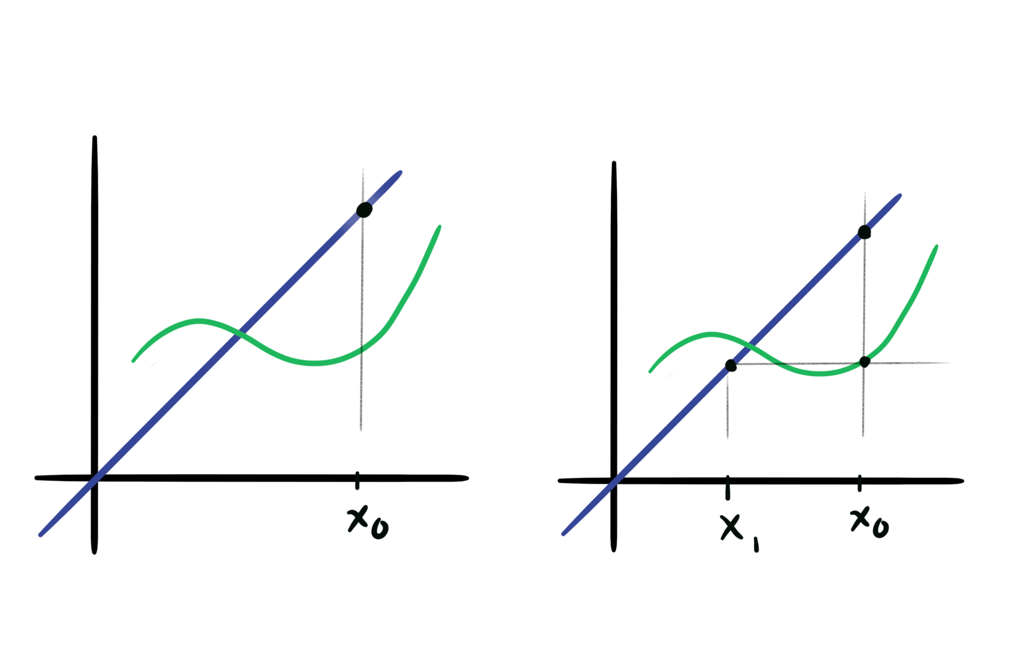
\includegraphics[width=0.85\textwidth]{FixedPoint}
                \caption{Paso de punto fijo}
            \end{figure}


        % ==============================================================
        % =================          IDEAS            ==================
        % ==============================================================
        \clearpage
        \subsection{¿Cómo eligo a $g(x)$?}

            Es muy sencillo, bueno, teorícamente. Sabes que $\Fun{x} = \FunG{x} - x = 0$,
            por lo tanto basta despejar y ver que: $\FunG{x} = x$.
            
            Es decir, toma a $\Fun{x} = 0$ y empieza a manipularla la expresión hasta
            que llegues de un lado la identidad y del otro lado lo que tendrás será a $g(x)$.

            Es decir tienes que llegar a $x = blob$ ó $x = g(x)$.

            

        % ==============================================================
        % =============        PROPIEDADES            ==================
        % ==============================================================
        \subsection{Propiedades}

            \begin{itemize}
                \item Sea $\Fun{x} = 0$ escrita de forma $\Fun{x} = \FunG{x} - x = 0$, es decir
                    $\FunG{x} = x$.

                    Entonces si $\forall x \in [\VarA, \VarB]$ se cumple que:
                    \begin{itemize}
                        \item $\FunG{x} \in [\VarA, \VarB]$
                        \item $\FunG{x}$ toma todos los valores entre $\VarA$ y $\VarB$
                        \item $\Color{\ColorFunG}{g'(x)}$ existe en $(\VarA, \VarB)$ y existe una constante $0 < r < 1$ tal que
                            $\Abs{\Color{\ColorFunG}{g'(x)}} \leq r$
                    \end{itemize}

                    Va a pasar que: 
                    \begin{itemize}
                        \item Existe un único punto fijo $x = \Root$ de $\FunG{x}$ entre $[\VarA, \VarB]$
                        \item La sequencia $\VarXpu = g(\VarX)$ converge siempre a $\Root$
                    \end{itemize}

            \end{itemize}


    % ===============================================================================
    % ===================              NEWTON                  ======================
    % ===============================================================================
    \chapter{Newton}

        % ==============================================================
        % =================          IDEAS            ==================
        % ==============================================================
        \clearpage
        \section{Definición}

            Resulta ser que el método de Newton se basa en el de punto fijo, es solo que 
            podemos elegir una $\FunG{x}$ muy especial, $\FunG{x} = x - \dfrac{\Fun{x}}{\FunDer{x}}$.

            Suponte que $\FunDerDer{x}$ existe, es continua sobre $[\VarA, \VarB]$ y $\Root$ una raíz simple
            de $\Fun{x}$ (es decir $\Fun{\Root} = 0$ y $\FunDerDer{\Root} \neq 0$).
            Entonces usar el método de punto fijo funcionará para hallar la raíz.

                        
        % ==============================================================
        % ===== =     DE DONDE SALIO ESTA FORMULA FUNCIONA      ========
        % ==============================================================
        \subsection{De donde salio esta fórmula}

            Busquemos un punto $x_0$ y supongamos que por ahí esta la raíz, entonces
            podemos sacar la ecuación de la recta tangente a ese punto como:
            \begin{MultiLineEquation*}{3}
                y - y_0 &= \FunDer{x_0} (x - x_0)                           \\
                \Fun{x} - \Fun{x_0} &= \FunDer{x_0} (x - x_0)             \\
                \Fun{x}  &= \FunDer{x_0} (x - x_0) + \Fun{x_0}        
            \end{MultiLineEquation*}
            
            Ahora busquemos el punto en el que $y = 0$, entonces:
            \begin{MultiLineEquation*}{3}
                \Fun{x}   &= \FunDer{x_0} (x - x_0) + \Fun{x_0}                     \\     
                0         &= \FunDer{x_0} (x - x_0) + \Fun{x_0}                     \\     
                - \Fun{x_0}  &= \FunDer{x_0} (x - x_0)                              \\     
                -\dfrac{\Fun{x_0}}{\FunDer{x_0}}     &= (x - x_0)                   \\     
                (x - x_0)  &= -\dfrac{\Fun{x_0}}{\FunDer{x_0}}                      \\     
                x         &= x_0 - \dfrac{\Fun{x_0}}{\FunDer{x_0}}     
            \end{MultiLineEquation*}

            Con esto llegamos la iteración de Newton:
            \begin{LargeEq}
                \begin{MultiLineEquation*}{3}
                    \VarXpu &= \VarX - \dfrac{\Fun{\VarX}}{\FunDer{\VarX}}     
                \end{MultiLineEquation*}
            \end{LargeEq}

        % ==============================================================
        % =============     PORQUE FUNCIONA           ==================
        % ==============================================================
        \clearpage
        \subsection{Porque funciona}

            Elegimos a:
            \begin{MultiLineEquation*}{3}
                \FunG{x} = x - \dfrac{\Fun{x}}{\FunDer{x}}
            \end{MultiLineEquation*}

            Entonces:
            \begin{MultiLineEquation*}{3}
                \Color{\ColorFunG}{g'(x)}
                    &= 1 - \dfrac{\FunDer{x}^2 - \Fun{x}\FunDerDer{x} }{\FunDer{x}^2}   \\
                    &= \dfrac{\Fun{x}\FunDerDer{x} }{\FunDer{x}^2} 
            \end{MultiLineEquation*}

            Entonces:
            \begin{MultiLineEquation*}{3}
                \Color{\ColorFunG}{g'(\Root)}
                    &= \dfrac{\Fun{\Root}\FunDerDer{\Root} }{\FunDer{\Root}^2}     \\
                    &= \dfrac{0 \FunDerDer{\Root} }{\FunDer{\Root}^2}     \\
                    &= 0   
            \end{MultiLineEquation*}

            Donde tenemos que $\Fun{\Root} = 0$ y $\FunDer{\Root} \neq 0$. 
            Entonces como $\Color{\ColorFunG}{g'(x)}$ es continua, entonces eso nos
            dice que existe una pequeña región cerca de la raíz en que 
            $\Abs{\Color{\ColorFunG}{g'(x)}} < 1$.

            Entonces si tomamos un punto inicial $x_0$ suficientemente cerca de la raíz, entonces
            las iteraciones de punto fijo estan garantizada a converger.


        % ==============================================================
        % =============           GEOMETRIA           ==================
        % ==============================================================
        \clearpage
        \subsection{Geometría}

            La interpretación de este método es tomar una estimación $\VarX$ entonces
            lo que hacemos es tomar la recta tangente a ese punto y ver donde es que la
            recta toca al eje $X$, ese será nuestra $\VarXpu$ y ve viendo que poco a poco lo
            que vamos haciendo es aproximarnos a la raíz.

            \begin{figure}[h]
                \centering
                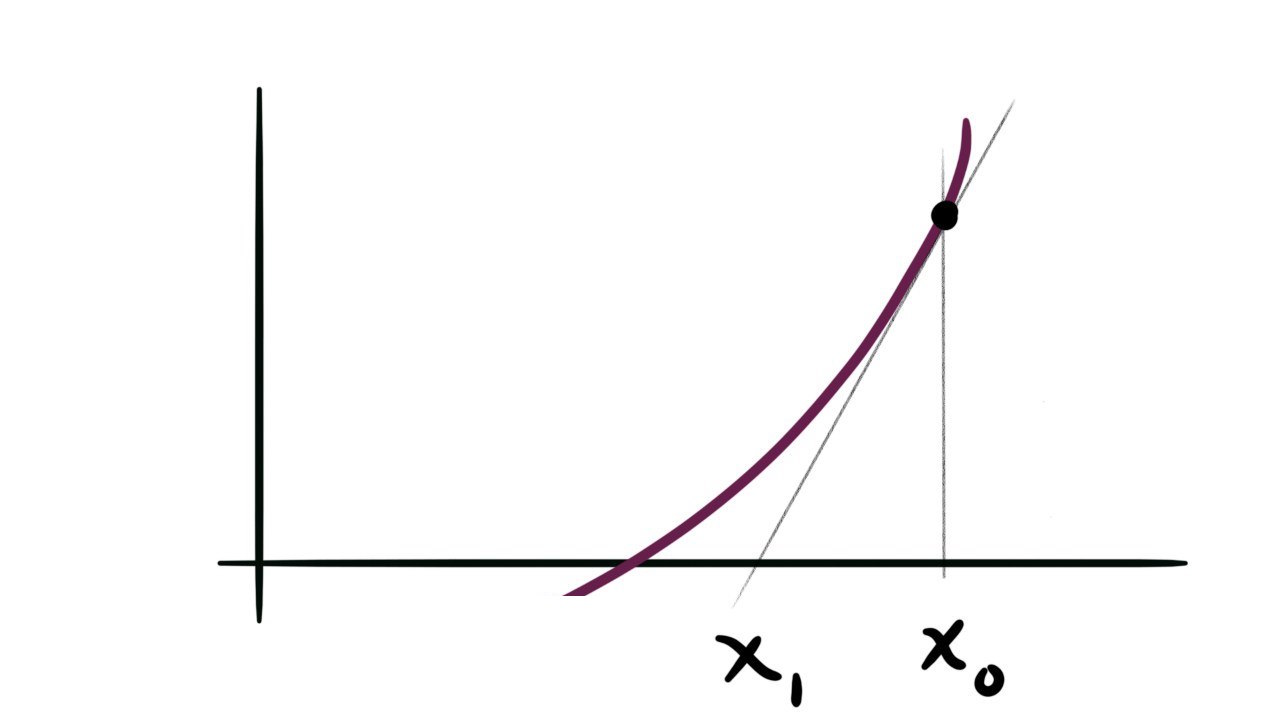
\includegraphics[width=0.65\textwidth]{Newton}
                \caption{Paso de punto fijo}
            \end{figure}

            
        % ==============================================================
        % ======              USARLO PARA SQRT(A)               ========
        % ==============================================================
        \subsection{Usar Newton para calcular la $\sqrt[n]{A}$}

            Si quieres calcular $\sqrt[n]{A}$ entonces puedes solucionar
            la ecuación $\Fun{x} = x^n - A = 0$.

            En ese caso $\FunDer{x} = n x^{n-1}$ y nuestra iteración es:
            \begin{LargeEq}
                \begin{MultiLineEquation*}{3}
                    \VarXpu 
                        &= \VarX - \dfrac{(\VarX)^n - A}{n (\VarX)^{n-1}}  
                         = \dfrac{(n-1)(\VarX)^n + A}{n (\VarX)^{n-1}} 
                \end{MultiLineEquation*}
            \end{LargeEq}



    % ===============================================================================
    % ===================              SECANTE                 ======================
    % ===============================================================================
    \chapter{Secante}

        % ==============================================================
        % =================          IDEAS            ==================
        % ==============================================================
        \section{Definición}

            Resulta ser que evaluar derivadas no suele ser super fácil :v
            Por lo tanto podemos aproximar la derivada como:
            \begin{MultiLineEquation*}{3}
                \FunDer{\VarX} \approx \dfrac{\Fun{\VarX} - \Fun{\VarXmu} }{\VarX - \VarXmu}
            \end{MultiLineEquation*}
            
            Entonces basta con esto para llegar a la iteración del método de secante:
            \begin{LargeEq}
                \begin{MultiLineEquation*}{3}
                    \VarXpu &= \VarX - \dfrac{\Fun{\VarX}(\VarX - \VarXmu)}{ \Fun{\VarX} - \Fun{\VarXmu} }     
                \end{MultiLineEquation*}
            \end{LargeEq}


    % ===============================================================================
    % ===================              REGLA FALSA             ======================
    % ===============================================================================
    \chapter{Regla Falsa}

    % ==============================================================
    % =================          IDEAS            ==================
    % ==============================================================
    \section{Definición}

        Aqui tenemos como dos estilos, bisección es perfecto en sentido de que una vez elegidos
        puntos iniciales validos, la raíz ya esta \Quote{encerrada} y con cada iteración solo mejoramos.

        Mientras que Newton y Secante con mucho mas rápidos pero si tomas puntos iniciales feos 
        estos métodos divergen y nunca tendrás una respuesta, de hecho cada iteración será peor.
        
        Así que este método es como un DLC en Secante con el objetivo de siempre estar seguro de
        que va a converger:

        % ==============================================================
        % =================          ITERACION            ==================
        % ==============================================================
        \subsection{Iteración}

            \begin{enumerate}
                \item Tienes dos puntos iniciales $(x_0, x_1)$ que encapsulen la raíz, puntos válidos para 
                    el método de bisección. 
                \item Ahora crea $x_2$ usando la iteración de la secante
                \item Ahora tienes 3 puntos, para elegir con cuales dos quedarte usa la idea
                    de bisección. Así de sencillo.
                \item Regresa al principio
            \end{enumerate}



% //////////////////////////////////////////////////////////////////////////////////////////////////////////
% /////////////////////                 SISTEMAS DE ECUACIONES               ///////////////////////////////
% //////////////////////////////////////////////////////////////////////////////////////////////////////////
\part{Aproximar Sistemas de Ecuaciones NO lineales}
\clearpage

    % ===============================================================================
    % ===================           TOLERANCIAS                ======================
    % ===============================================================================
    \chapter{Ideas generales de ceros de funciones}

        % ==============================================================
        % =================          IDEAS            ==================
        % ==============================================================
        \section{Ideas}

            Esto es sencillo, lo que tienes que hacer si es que tienes un montón de
            ecuaciones raras a las que quieres encontrar solución basta con tomar
            tu sistema e igualarlo a cero.

            Y ahora lo que estas viendo es nada más y nada menos que una función
            vectorial, que toma todos tus parametros y te regresa un vector columna
            de todas tus ecuaciones evaluadas en ese punto.

            Así que resolverlas es tan sencillo como encontrar una raíz dentro de 
            una función vectorial.
            

    % ===============================================================================
    % ===================           NEWTON                     ======================
    % ===============================================================================
    \chapter{Newton Generalizado}

        % ==============================================================
        % =================          IDEAS            ==================
        % ==============================================================
        \clearpage
        \section{Ideas}

            Recuerda que la iteración de Newton es:
            \begin{LargeEq}
                \begin{MultiLineEquation*}{3}
                    \VarXpu 
                        &= \VarX - \dfrac{\Fun{\VarX}}{\FunDer{\VarX}}     
                        &= \VarX - \FunDer{\VarX}^{-1} \Fun{\VarX}      
                \end{MultiLineEquation*}
            \end{LargeEq}

            Por lo tanto la idea de Newtons generalizado es
            que si $\BigFun{x}: \Reals^n \to \Reals^n$:
            \begin{LargeEq}
                \begin{MultiLineEquation*}{3}
                    \Over \VarXpu  
                        &= \Over \VarX - J_F\Wrap{\Over \VarX}^{-1} \BigFun{\Over \VarX}      
                \end{MultiLineEquation*}
            \end{LargeEq}

            Espera, espera, que demonios es $J_F$ te preguntaras, pues, es el Jacobiano,
            es una matriz que representa \Quote{la derivada de la función $\BigFun{x}$}.

            Pero, como te darás cuenta no solo hay que calcular el Jacobiano, sino que
            hay que evaluarlo y después invertir la matriz que nos da, y eso, pequeño ser
            humano no es fácil, así que podemos expresar la iteración de otra manera:
            \begin{LargeEq}
                \begin{MultiLineEquation*}{3}
                    \Over \VarXpu  
                        &= \Over \VarX + \Over S_k    
                \end{MultiLineEquation*}
            \end{LargeEq}

            Donde $\Over S_k$ como la solución al sistema:
            \begin{LargeEq}
                \begin{MultiLineEquation*}{3}
                    J_F(\Over \VarX) \Over S_k = - \BigFun{\Over \VarX} 
                \end{MultiLineEquation*}
            \end{LargeEq}

            





% //////////////////////////////////////////////////////////////////////////////////////////////////////////
% /////////////////////                  INTERPOLANTES                       ///////////////////////////////
% //////////////////////////////////////////////////////////////////////////////////////////////////////////
\part{Interpolantes}
\clearpage


    % ===============================================================================
    % ===================           IDEAS GENERALES            ======================
    % ===============================================================================
    \chapter{Ideas Generales}

        % ==============================================================
        % =================          DEFINICION       ==================
        % ==============================================================
        \clearpage
        \section{Definición}

            Suponte que existe una función ($\Fun{x}$) que queremos conocer, pero que no conocemos :(
            Lo único que tienes es un montón de puntos ($x_i$) y  el valor de la función en ese punto ($y_i$).

            Lo que haremos en este cápitulo será aproximar a esa función en un intervalo.


    % ===============================================================================
    % ===================    INTERPOLANTE LINEAL               ======================
    % ===============================================================================
    \chapter{Interpolante Lineal}

        % ==============================================================
        % =================          DEFINICION       ==================
        % ==============================================================
        \section{Definición}

            Lo único que hacemos es aproximar la función como un montón de lineas, y bueno, no hay mucho
            más que decir.

            El interpolante esta dado por:
            \begin{MultiLineEquation*}{3}
                I(x) := I(x_i) = y_i + \dfrac{x_{i+1} - x_i}{y_{i+1} - y_i}(x - x_i)
            \end{MultiLineEquation*}

            \begin{figure}[h]
                \centering
                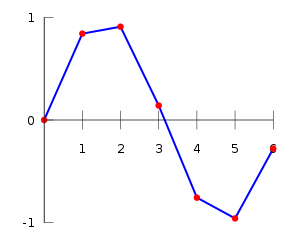
\includegraphics[width=0.45\textwidth]{LinealInterpolation}
                \caption{Ejemplo de como se ve}
            \end{figure}

    
    % ===============================================================================
    % ===================    INTERPOLANTE GRADO N              ======================
    % ===============================================================================
    \chapter{Interpolante Grado N}

        % ==============================================================
        % =================          DEFINICION       ==================
        % ==============================================================
        \section{Definición}

            Es la idea clásica, es suponer que la función que estamos buscando es un polinomio de grado $n$,
            en cuyo caso basta con hacer la clásica matriz de Vandermonde y resolver por mínimo cuadrados y
            obtendremos los coeficientes que estamos buscando.



    % ===============================================================================
    % ===================    INTERPOLANTE DE LAGRANGE          ======================
    % ===============================================================================
    \chapter{Interpolante de Lagrange}

        % ==============================================================
        % =================          DEFINICION       ==================
        % ==============================================================
        \clearpage
        \section{Definición}

            La idea es basicamente la misma, si tenemos $n$ puntos y sus valuaciones entonces
            podemos facilmente ver que existe un solo polinomio de grado $n$ que pasa por esos
            puntos. Justo como en el interpolante pasado, pero la diferencia en como obtenemos dicho
            polinomio.

        % ==============================================================
        % =================          POLINOMIO        ==================
        % ==============================================================
        \section{Polinomio de Langrange}

            El polinomio de Langrange esta asociado a un punto en especial de nuestro conjunto
            de puntos. Tiene que cumplir que:
            \begin{itemize}
                \item Para un $x_i$ tenemos que $L_i(x_i) = 1$
                \item Para un $x_j$ tal que $i \neq j$, entonces $L_j(x_i) = 0$
            \end{itemize}

            Veamos como sería para el caso de los puntos:

            % ======== EJEMPLO ========
            \begin{SmallIndentation}[1em]
                \textbf{Ejemplo}:
            
                Suponte que tenemos dos puntos ($x_0, y_0$) y ($x_1, y_1$).
                Entonces lo que queremos es un polinomio que evaluado en esos puntos de
                lo que tiene que dar y de grado 2. Es sencillo:
                \begin{MultiLineEquation*}{3}
                    L_0(x) = \dfrac{x - x_1}{x_0 - x_1}
                    \MegaSpace
                    L_1(x) = \dfrac{x - x_0}{x_1 - x_0}
                \end{MultiLineEquation*}

                Entonces el interpolante es tan sencillo como:
                \begin{MultiLineEquation*}{3}
                    I(x) := f(x_0) \; L_0(x) + f(x_1) \; L_1(x)
                \end{MultiLineEquation*}

            \end{SmallIndentation}

            Siendo generales tenemos que:
            \begin{itemize}
                    \item 
                        Un polinomio de Lagrange:
                        \begin{MultiLineEquation*}{3}
                            L_k(x) := \prod_{i = 0, i \neq k} \dfrac{x - x_i}{x_k - x_i}
                        \end{MultiLineEquation*}
                        
                    \item 
                        Nuestro interpolante:
                            \begin{MultiLineEquation*}{3}
                                I(x) := f(x_0) \; L_0(x) + f(x_1) \; L_1(x) + \dots + f(x_n) \; L_n(x)
                            \end{MultiLineEquation*}
            \end{itemize}
                
    % ===============================================================================
    % ===================    INTERPOLANTE DE NEWTON            ======================
    % ===============================================================================
    \chapter{Interpolante de Newton}

        % ==============================================================
        % =================          DEFINICION       ==================
        % ==============================================================
        \clearpage
        \section{Definición}

            La idea es basicamente la misma, si tenemos $n$ puntos y sus valuaciones entonces
            podemos facilmente ver que existe un solo polinomio de grado $n$ que pasa por esos
            puntos. Justo como en el interpolante pasado, pero la diferencia en se vera dicho interpolante.

            Queremos que se vea como:
            \begin{MultiLineEquation*}{3}
                I(x) := a_0
                        + a_1 (x-x_0)
                        + a_2 (x-x_0)(x-x_1)
                        + \dots
                        + a_n (x-x_0)(x-x_1)\dots(x-x_{n-1})
            \end{MultiLineEquation*}

            Ahora todo lo que necesitamos saber es como sacar esos coeficientes.

        % ==============================================================
        % ===========         DIFERENCIAS DIVIDIDAS    =================
        % ==============================================================
        \clearpage
        \section{Diferencias Divididas}

            Decimos que la i-ésima diferencia dividida de orden cero es:
            \begin{MultiLineEquation*}{3}
                f[x_i] = f(x_i)
            \end{MultiLineEquation*}
            
            Denotamos la i-ésima diferencia dividida de primer orden como:
            \begin{MultiLineEquation*}{3}
                f[x_i, x_{i+1}] = \dfrac{f[x_{i+1}] - f[x_i]}{x_{i+1} - x_i}
            \end{MultiLineEquation*}

            Por lo tanto podemos generalizar y decir que:
            \begin{MultiLineEquation*}{3}
                f[x_i \dots, x_j]
                    := \dfrac{ f[x_{i+1}, \dots, x_j] - f[x_i, \dots, x_{j-1}] }{ f(x_j) - f(x_i) }
            \end{MultiLineEquation*}
            
            Y lo mas genial ahora es que podemos mostrar el interpolante es:
            \begin{MultiLineEquation*}{3}
                I(x) := f[x_0] + \sum_{k = i}^n f[x_0, x_1, \dots, x_k](x-x_0)(x-x_1)\dots(x-x_{k-1})
            \end{MultiLineEquation*}
            


            

% //////////////////////////////////////////////////////////////////////////////////////////////////////////
% /////////////////////                  OPTIMIZACION                        ///////////////////////////////
% //////////////////////////////////////////////////////////////////////////////////////////////////////////
\part{Optimización}
\clearpage

    % ===============================================================================
    % ===================             SECCION AUREA            ======================
    % ===============================================================================
    \chapter{Sección Áurea}

        % ==============================================================
        % =================          DEFINICION       ==================
        % ==============================================================
        \clearpage
        \section{Unimodal}

            Tomemos una función unimodal $\Fun{x} : \Reals \to \Reals$ dentro de un rango
            $[\VarA, \VarB]$.

            Decir que es unimodal es decir que la función antes del mínimo siempre 
            decrece y después del mínimo siempre crece.

            O más formalmente tenemos que:
            \begin{itemize}
                \item $\forall \VarXOne, \VarXTwo$ tal que 
                    $\VarXOne < \VarXTwo < minimo$ entonces $\Fun{\VarXOne} > \Fun{\VarXTwo}$ 
                \item $\forall \VarXOne, \VarXTwo$ tal que 
                    $minimo < \VarXOne < \VarXTwo$ entonces $\Fun{\VarXOne} < \Fun{\VarXTwo}$ 
            \end{itemize}

            
        % ==============================================================
        % =================          ALGORITMO        ==================
        % ==============================================================
        \section{Algoritmo}

            Toma un segmento en el que nuestra función $\Fun{x}$ es unimodal. Llamemoslo $[\VarA, \VarB]$.

            Entonces definimos:
            \begin{itemize}
                \item $\tau = \dfrac{\sqrt{5}-1}{2} = 0.618$
                \item $1 - \tau = 0.382$
                \item $\VarXOne = \VarA + (1-\tau)(\VarB - \VarA)$
                \item $\VarXTwo = \VarA + (\tau)  (\VarB - \VarA)$
            \end{itemize}

            Con esta definición creo que es fácil probar que $\VarA < \VarB$

            Ahora, pueden pasar dos cosas:

            \begin{multicols*}{2}
                \begin{itemize}
                    \item $\Fun{\VarXOne} < \Fun{\VarXTwo}$:

                        Entonces estamos seguros de que el mínimo no puede estar en el segmento 
                        $[\VarXTwo, \VarB]$ porque como vimos es una función unimodal.

                        Por esto mismo tomamos que:
                        \begin{itemize}
                            \item $\VarB = \VarXTwo$
                            \item $\VarXTwo = \VarXOne$
                            \item $\VarXOne = \VarA + (1-\tau)(\VarB - \VarA)$
                        \end{itemize}

                    \ForceColumnBreak

                    \item $\Fun{\VarXOne} > \Fun{\VarXTwo}$:

                    Entonces estamos seguros de que el mínimo no puede estar en el segmento 
                    $[\VarA, \VarXOne]$ porque como vimos es una función unimodal.

                    Por esto mismo tomamos que:
                        \begin{itemize}
                            \item $\VarA = \VarXOne$
                            \item $\VarXOne = \VarXTwo$
                            \item $\VarXTwo = \VarA + (\tau)(\VarB - \VarA)$
                        \end{itemize}

                \end{itemize}
            \end{multicols*}
            






\end{document}